%!TEX root = ../Main.tex

\chapter{Introduction}

%It defines the objectives and the importance of the research. It focus on the the application of Next Generation Sequencing to molecular biology, wheat genetics and ultimately to breeding programs. It also mentions the current status of the wheat reference genome and other resources (genetic maps, markers) the need of tools to query them effectively. 

In order to produce bioinformatic software that is powerful and usable it is required an understanding of both: the biological processes to solve and; the computational methods and software development practices.

\begin{landscape}
 \begin{figure}
  \centering
  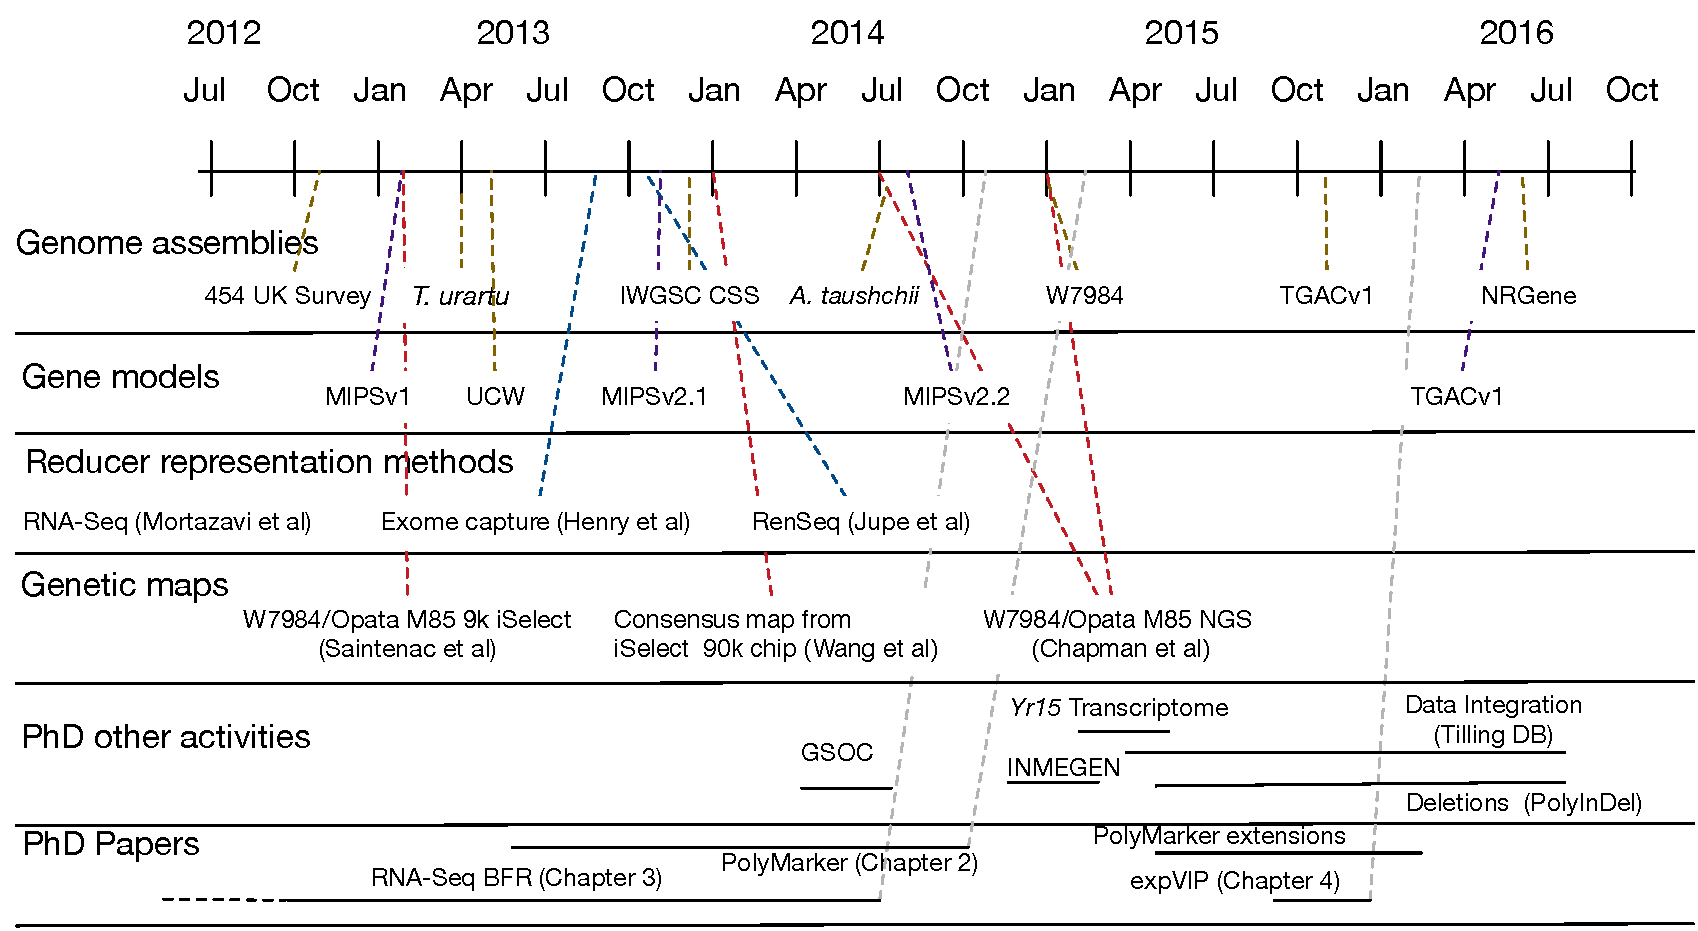
\includegraphics[height=0.9\textheight]{Introduction/RicardoPhdTimelineV1.pdf}
  \caption{Timeline of the projects carried on during this PhD and the wheat resources that were released in the same period of time. }
  \label{fig:intro:timeline}
 \end{figure}
\end{landscape}